\documentclass[a4paper,upLaTeX,luatex,12pt]{ltjsarticle}
\usepackage[utf8]{inputenc}
\usepackage{fancyhdr}
\usepackage[top=25truemm,bottom=20truemm,left=20truemm,right=20truemm]{geometry}
\usepackage[listings]{tcolorbox}
\usepackage{ascmac}
\usepackage{amsmath} %数式
\def\Date{2023/5/23}
\def\ClassNum{}
\def\Subject{}

\pagestyle{fancy}
\rhead{\textbf{\Date}}
\lhead{\textbf{ロジスティック回帰}}
\cfoot{}
\rfoot{担当:鈴木柾孝} %これおk?

\begin{document}
\section{ロジスティック回帰とは}
ロジスティック分析は、ある事件(event)が発生するかしないかを直接予測することではなく、その事件が発生する確率を予測する。\textbf{従って、被説明変数の値は0と1の間の数値になる。}分析結果、被説明変数の値、すなわち確率が0.5より大きいとその事件が発生すると予測し、0.5を下回るとその事件が発生しないと予測する。\par
つまり,\textbf{ロジスティック回帰は,ある事象が発生する確率を予測するための手法である.または,クラスに分類分けするためのものである.}\par
ロジスティック回帰を行うときは,説明変数が年収などの量的データで,被説明変数が「ある事象が発生するかしないか」のような質的データ(ex.車持ってるか)であることが多い.\par
このように被説明変数が質的データであっても分析ができるよう一般線形モデルを拡張したのが一般化線形モデル(GLM:Generalized Linear Model)である。
\begin{figure}[htbp]
  \centering
  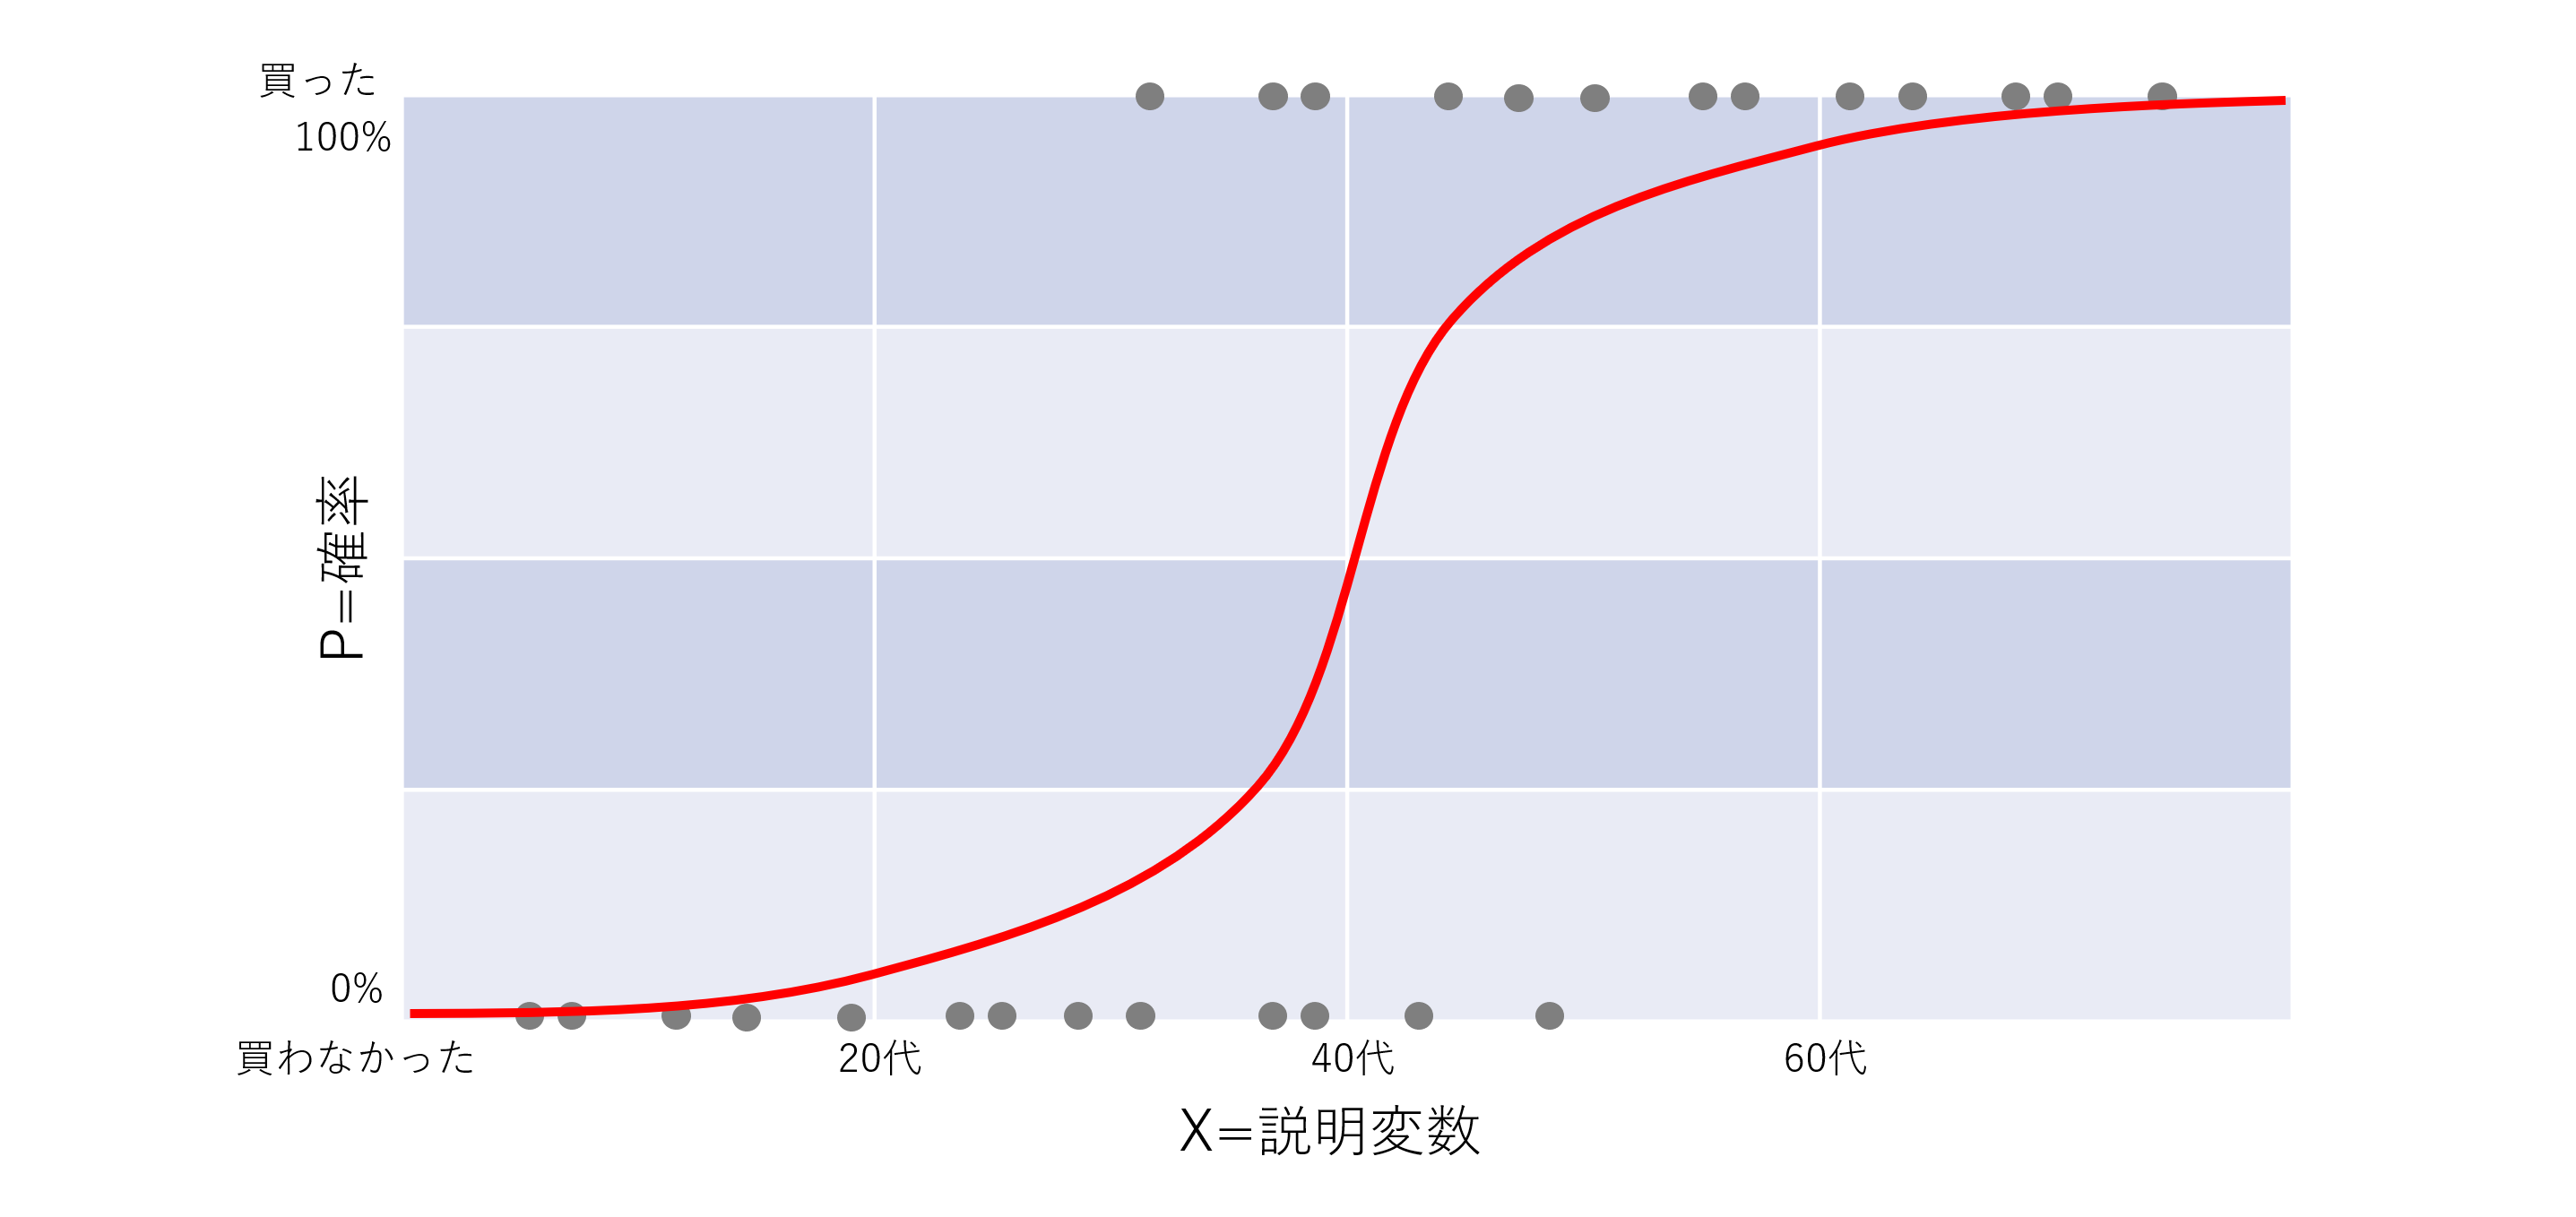
\includegraphics[width=0.9\linewidth]{/Users/masataka/Coding/Pythons/WDSC 2023/Study for machine learning/ロジスティック回帰/assets/image-12.png}
  \caption{ロジスティック回帰の例}
  \label{fig:}
\end{figure}
\section{ロジスティック回帰の注意点}
ロジスティック回帰で解析するべきものを線形回帰で解析すると,誤った結果が出てしまう.\par
つまり,0-1の間の値をとるべきなのに,それを超えて0未満や1より大きい値をとってしまう.\par
\section{オッズとオッズ比}
オッズとは,ある事象が起こる確率と起こらない確率の比のことである.\par
\begin{equation}
  オッズ=\frac{起こる確率}{起こらない確率}= \frac{p}{1-p}
\end{equation}
オッズの値は,0から無限大までの値をとることに注意する.\par
一方,オッズ比は,ある事象が起こる確率のオッズと,別の事象が起こる確率のオッズの比のことである.\par
\begin{equation}
  オッズ比=\frac{\frac{p_1}{1-p_1}}{\frac{p_2}{1-p_2}}
\end{equation}
例えばオッズ比を利用すると、自動車を所有している世帯主が自動車を所有していない世帯主に比べて何倍住宅を所有しているかが計算できる。\par
ここで,注意しないといけないのが,オッズ比が1より小さいときである.例えば,「0.01倍増加する」という結果が得られたとき,これは減少しているということであることに気をつけたい.\par
\section{ロジスティック回帰を使うとき}
ロジスティック回帰に適しているのは、求めたい目的変数が明確なシーンである。購入の有無、台風・落雷が発生するかしないか、病気に罹るか罹らないかなどの予測にはロジスティック回帰が向いている。
逆に目的変数が曖昧なときや、数値を知りたいときにはロジスティック回帰は向いない。
\section{ロジット関数}
ロジスティック回帰は,\textbf{線形回帰の結果を0-1の間に収めるため}に,ロジット関数を用いる.\par
\begin{equation}
  ロジット関数=logit(p)=log\frac{p}{1-p}
\end{equation}
ロジット関数は,オッズの対数をとったものである.\par
\section{ロジスティック回帰の式}
回帰において,連続的な値に対してはax+bというのがもとまる.しかし,今回のように\textbf{離散的}な値を取るにはこれを変える必要がある.
そこで登場するのが\textbf{リンク関数}で,ロジスティック回帰には,ロジット関数を使う.(一般化回帰には必須?)
(リンク関数によって,\textbf{連続的な値を離散的な値に変換する}ことができるってことだと思う)\par
\begin{align}
  log\frac{p}{1-p}  & =ax+b                             \\
  \Leftrightarrow p & =\frac{1}{1+e^{-(ax+b)}} ←図1みたいな式
\end{align}
Pythonで計算した後に出てくる切片と傾きは,この式のaとbだと思われる.\par
\section{評価}
分類系のものの評価は,Confusion Matrixを用いるのが良いそう.(大森先生より)\par
\section{ロジスティック回帰の種類}
\subsection{二項ロジスティック回帰}
二項ロジスティック回帰は,被説明変数が2値の場合に用いられる.\par
\subsection{多項ロジスティック回帰}
多項ロジスティック回帰は,被説明変数が3値以上の場合に用いられる.\par
\subsection{順序ロジスティック回帰}
順序ロジスティック回帰は,被説明変数が3値以上の場合に用いられるが,それらに順位がある場合に用いられる.\par
\end{document}